\renewcommand{\lecturetitle}{NAS-Bench-101: The first NAS benchmark}
\renewcommand{\lecturetime}{Week 9, Video 4}
\section{\lecturetitle}
%-------------------------------------------------
%-------------------------------------------------

%----------------------------------------------------------------------
\myframe{Reproducibility crisis in NAS and the necessity of NAS benchmarks}{

\myit{
	\item \textit{\color{red}{Problem:}} Most of the NAS methods we saw so far are \alert{extremely difficult to reproduce and compare} (see \lit{\href{https://arxiv.org/pdf/1902.07638.pdf}{Li \& Talwalkar, 2019}; \href{https://arxiv.org/pdf/1909.02453.pdf}{Lindauer \& Hutter, 2020}}) due to:
	\myit{
		\item[--] Different search spaces
		\item[--] Different training pipelines
		\item[--] Other confounding factors such as different hardwares, different deep learning library versions, etc.
		\item[--] Industry-scale computational resources are not accessible to everyone	
		\item[--] No publicly available code
	}
\pause
\medskip
	\item \textit{\color{red}{Solution:}} A benchmark for NAS methods
}


\begin{center}
\begin{minipage}{0.8\textwidth}
\begin{block}{Definition: NAS Benchmark \lit{\href{https://arxiv.org/pdf/1909.02453.pdf}{Lindauer \& Hutter, 2020}}}
\textit{A NAS benchmark consists of a dataset (with a predifiend training-test split), a search space, and available runnable code with pre-defined hyperparameters for training the architectures.}
\end{block}
\end{minipage}
\end{center}

}
%-----------------------------------------------------------------------

%----------------------------------------------------------------------
\myframe{NAS-Bench-101: The first NAS benchmark \litw{\href{http://proceedings.mlr.press/v97/ying19a.html}{Ying et al, 2018}}}{

\centering
\myit{
	\item Cell-structured search space consisting of all directed acyclic graphs (DAGs) on $V=5$ nodes, where each possible node has $L$ operation choices.
	\pause
	\item To limit the number of architectures, NAS-Bench-101 has the following constraints:
	\myit{
		\item $L = 3$:
			\begin{columns}
			\column{.18\textwidth}
			- $3 \times 3$ convolution
			\column{.18\textwidth}
			- $1 \times 1$ convolution
			\column{.2\textwidth}
			- $3 \times 3$ max-pooling			
			\end{columns}
		\item $V \leq 7$
		\item A maximum of 9 number of edges
	}
}

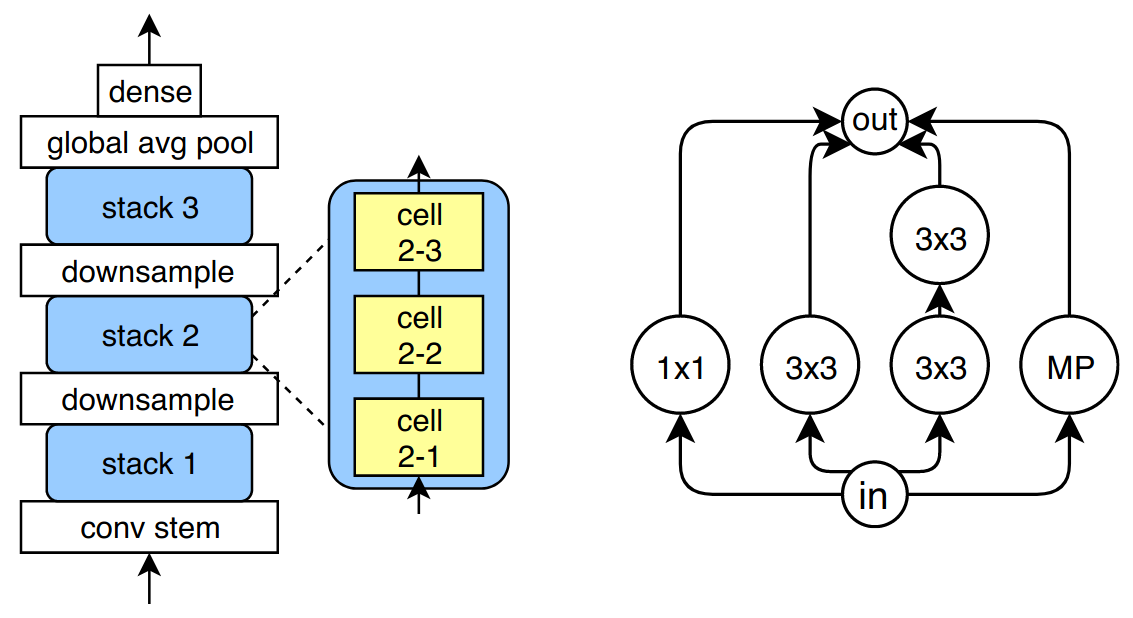
\includegraphics[width=.5\textwidth]{images/nasbench101_graph.png}

}
%-----------------------------------------------------------------------

%----------------------------------------------------------------------
\myframe{NAS-Bench-101: The first NAS benchmark \litw{\href{http://proceedings.mlr.press/v97/ying19a.html}{Ying et al, 2018}}}{

\centering
\myit{
	\item Exhaustively trained and evaluated all possible models on CIFAR-10 to create a tabular (queryable) benchmark
	\pause
}

\begin{columns}
\column{.6\textwidth}
\vspace{-3.2cm}
\myit{
	\item around 423k \alert{unique} cells
	\myit{
		\item[--] 4 epoch budgets: 4, 12, 36, 108
		\item[--] 3 repeats
		\item[--] around 5M trained and evaluated models
		\item[--] 120 TPU years of computation
		\item[--] the best architecture mean test accuracy: 94.32\%
		}
	\medskip
	\item Given an architecture encoding $A$, budget $E_{stop}$ and trial number, one can query from NAS-Bench-101 the following quantities:
	\myit{
		\item[--] training/validation/test accuracy
		\item[--] training time in seconds
		\item[--] number of trainable model parameters
		}
}

\column{.36\textwidth}
%\vspace{-3cm}
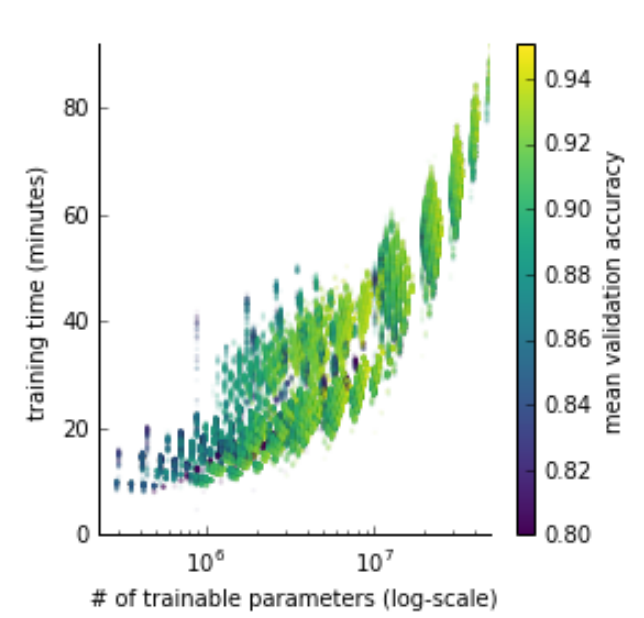
\includegraphics[width=.63\textwidth]{images/nasbench101_stat1.png}\\
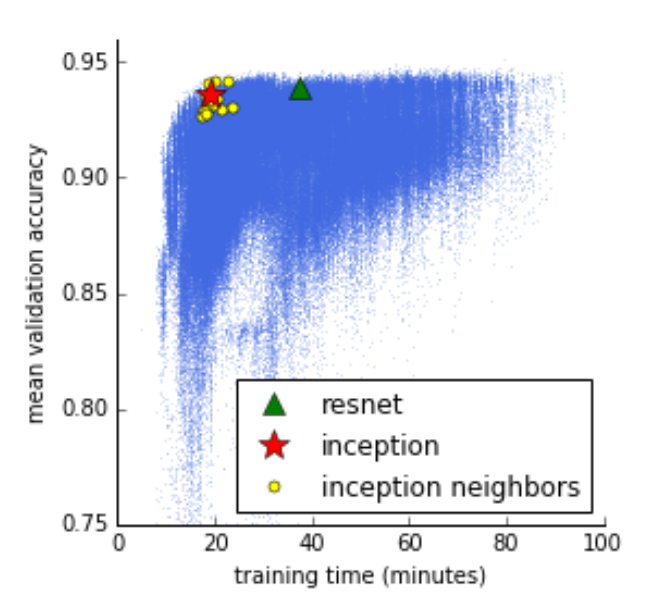
\includegraphics[width=.66\textwidth]{images/nasbench101_stat2.png}
\end{columns}

}
%-----------------------------------------------------------------------

%----------------------------------------------------------------------
\myframe{Blackbox NAS Methods on NAS-Bench-101 \litw{\href{http://proceedings.mlr.press/v97/ying19a.html}{Ying et al, 2018}}}{
	\myit{
%		\item All methods find good architectures
		\item RL outperforms random search
		\item BO and regularized evolution perform best, better than RL
	}
	\centering
	\medskip
	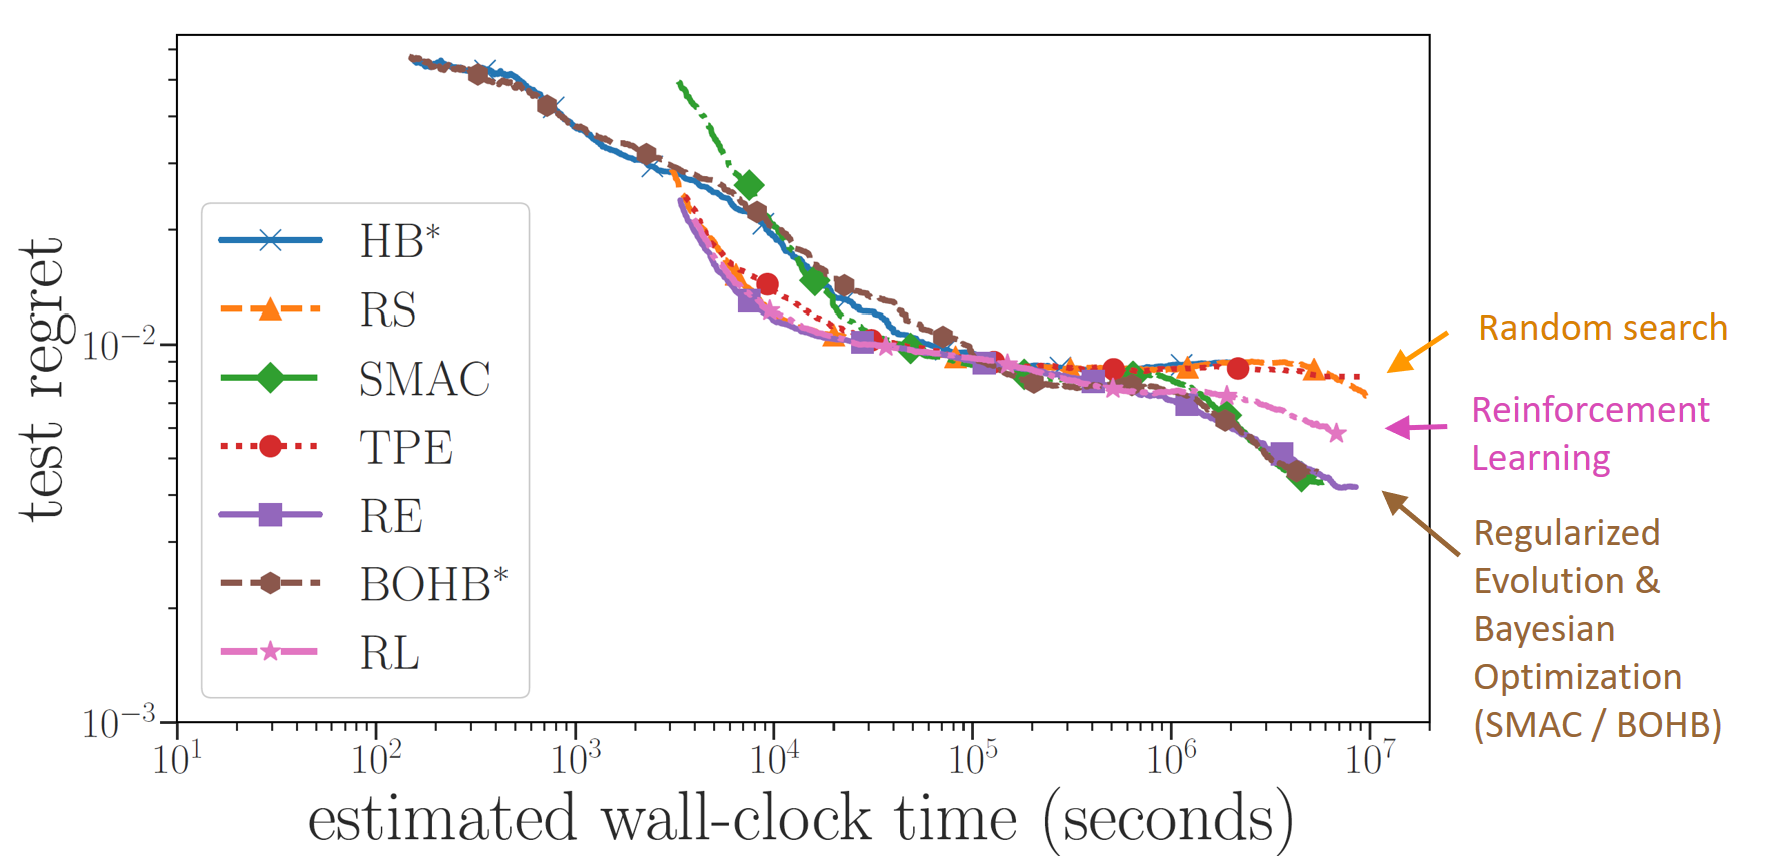
\includegraphics[width=.6\textwidth]{images/NAS-Bench-101-results-with-labels}

\pause
	\myit{
		\item Note that the BO method SMAC \lit{\href{https://link.springer.com/chapter/10.1007/978-3-642-25566-3_40}{Hutter et al, 2011}} predated RL for \\NAS \lit{Zoph \& Le, 2017} by 6 years
		\myit{
			\item[-] Only now, benchmarks like NAS-Bench-101 allow for efficient comparisons
		}
	}
}
%-----------------------------------------------------------------------

%----------------------------------------------------------------------
\myframe{Questions to Answer for Yourself / Discuss with Friends}{

	\myit{
		\item Repetition:\\ 
		\alert{Why do we need proper benchmarking of NAS algorithms?}
		\item Repetition:\\
		\alert{What does a NAS benchmark subsume?}
	}	 
}
%-----------------------------------------------------------------------